% Chapter Template

\chapter{DMN and It's identification with EEG} % Main chapter title

\label{Chapter 1} % Change X to a consecutive number; for referencing this chapter elsewhere, use \ref{ChapterX}

\lhead{Chapter 1. \emph{DMN and It's identification with EEG}} % Change X to a consecutive number; this is for the header on each page - perhaps a shortened title

%----------------------------------------------------------------------------------------
%	SECTION 1
%---------------------------------------------------------------------------------------
\section{Introduction}



The brain is made up largely of cortical networks Which are intrinsically linked to higher levels of cognition . In these networks, the default mode network (DMN), which includes the precuneus/posterior cingulate cortex, Medial prefrontal cortex, and temporoparietal junction,Is of special interest, as it has been linked to neuropsychiatric for ropsychiatric disorders  and degree of consciousness.
 
A variety of neuroimaging techniques have been used to analyze the DMN. Functional Magnetic Resonance Imaging (fMRI) or Positron Emission Tomography (PET) are routinely used to identify the DMN, either by contrasting resting-state to task-induced DMN deactivation levels or by a functional connectivity analysis on resting-state recordings. Several attempts have been also made to recover the DMN from magnetoencephalographic recordings (MEG). Using resting-state data, There are some researchers who identified MEG correspondents of DMN with a topography of inter-regional band power correlations in the $\theta$- (3.5–7 Hz), $\alpha$ - (8–13 Hz), and $\beta$- (14–25 Hz) band. And identified MEG signatures of DMN activity by amplitude envelope correlations in the $\alpha$-band (8–13 Hz).

However, fMRI, PET and MEG are difficult to perform on certain groups of patients, such as severely paralysed patients in late stages of amyotrophic lateral sclerosis (ALS), that are dependent on artificial ventilation systems and thus cannot be easily put into the MRI, PET, or MEG scanners. In contrast, EEG is a portable, safe (non-invasive), cheap, and widespread technology, that can be used at the patient’s home. EEG-based DMN characterisation would enable the investigation of alterations in DMN activity in a wide range
of patients groups that are difficult to examine with other methods. In particular, the connectivity within the DMN is negatively correlated with the degree of consciousness impairment and thus could be used to distinguish the conscious state from the vegetative state in CLIS  patients, for whom the degree of consciousness cannot be concluded from behaviour due to the absence of communication.

we devised a new technique to identify EEG-based DMN pattern more similar to regions identified by fMRI. we are using data during during an another research project of identifying mind wandering and alert state by analyzing $\theta$ ,$\alpha$ ,$\beta$ ,$\gamma$ and $\delta$ band frequency.

\subsection{Literature Survey}

Although there are many methods are available these days to identify default mode network, not all are appropriate for all group of people. With fMRI or PET , we can easily identify DMN but there are limited patients that we can examine with fMRI or PET. So, we tried to develop topological graph of head using EEG.
According to a paper on "Functional connectivity in the resting brain:A network analysis of the default mode hypothesis" by Michael D. Greicius, Ben Krasnow, Allan L. Reiss and Vinod Menon,the default mode network is thought to be most active during the resting state, it may also persist during passive sensory processing states. To explore this possibility, they generated connectivity maps for the PCC and the vACC during their visual processing task and compared them to the resting-state maps. The PCC and vACC maps were virtually identical in the resting state and the visual processing task, suggesting that the default mode neural network is minimally disrupted by sensory processing tasks with limited cognitive demand. It is important to note, in this regard, that the PCC and vACC were not ‘‘deactivated’’ in the visual processing task, further suggesting similar levels of ongoing activity in the default mode network during the flashing and still checkerboard epochs.
\begin{figure}
    \centering
    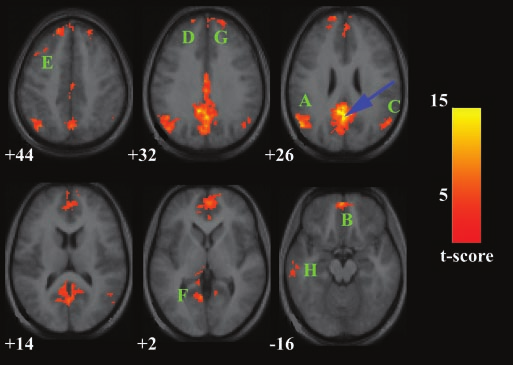
\includegraphics[height=5cm]{Pictures/fmri.png}
    \caption{Map of the resting-state neural connectivity for the PCC. The blue arrow indicates the approximate location of the PCC peak.}
    \label{fig5}
\end{figure}

\begin{figure}
    \centering
    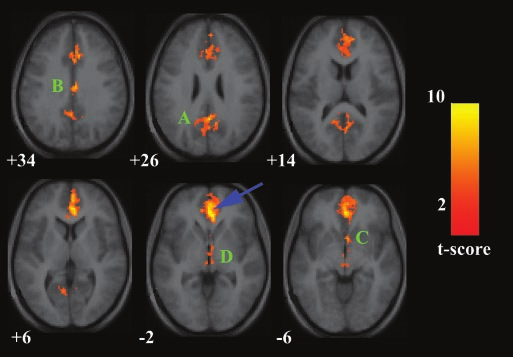
\includegraphics[height=5cm]{Pictures/fmri1.png}
    \caption{Map of the resting-state neural connectivity for the vACC. The blue arrow indicates the approximate location of the vACC maximum.}
    \label{fig6}
\end{figure}

\subsection{Research gaps}
    The DMN is routinely identified with functional magnetic resonance imaging (fMRI) or positron emission tomography (PET). However, both of these methods impose restrictions on the groups of patients that can be examined.Since, fMRI is not portable, and too expensive ,our work enables the characterization of DMN alterations in patient groups that are difficult to study with fMRI or PET

\subsection{Objective}
    The objective of my project is to show that the DMN can also be identified by electroencephalography (EEG). By instructing subjects to alternate between self-referential memory recall and focusing on their breathing induces a spatial pattern of spectral band power modulation in the $\theta$- and $\alpha$-band (4–16 Hz) that is consistent with the DMN pattern observed with PET and fMRI.
    In my study, i have developed a topological graph of head to show the activated brain regions during mind wandering state. 

\section{Default Mode Network in brain}
    Default mode network (DMN) is a large scale brain network of interacting brain regions known to have activity highly correlated with each other.DMN is most commonly active when a person is not focused on the outside world and the brain is at wakeful rest, such as during daydreaming and mind-wandering.Also active when the individual is thinking about others, thinking about themselves, remembering the past, and planning for future.The DMN has been shown to be negatively correlated with other networks in the brain such as attention networks.Fig 1.3 shows the parts for brain active during mind wandering state also called DMN.
    \begin{figure}
        \centering
        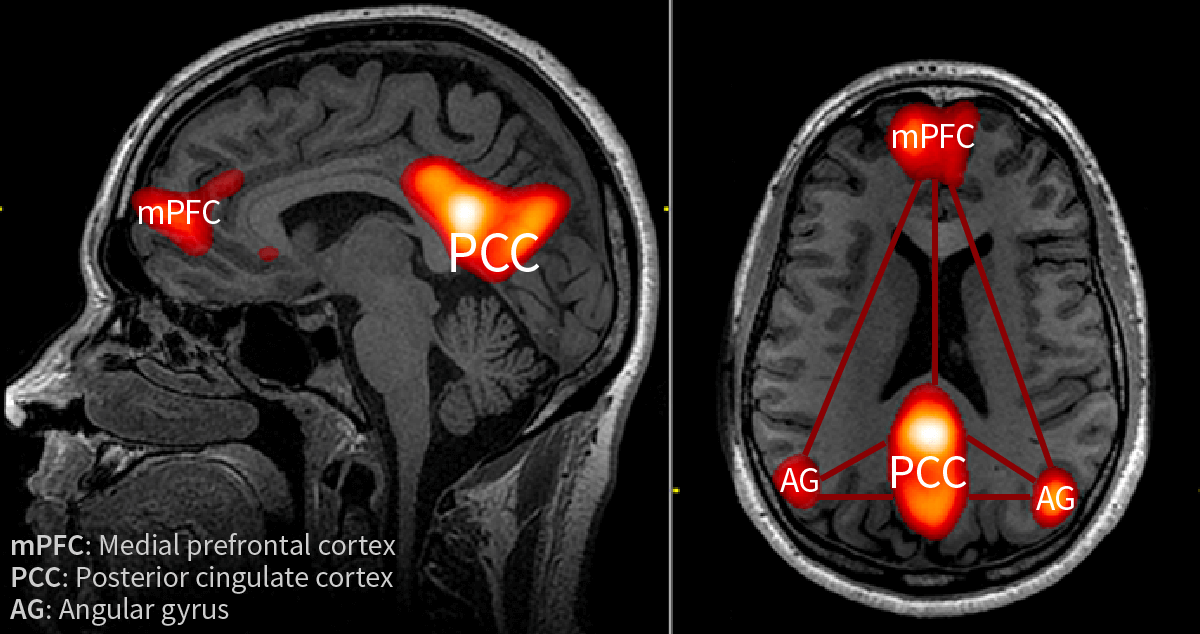
\includegraphics[height=7cm]{Pictures/dmn.png}
        \caption{fMRI scan showing default mode network [2]}
        \label{fig:my_label2}
    \end{figure}
\subsection{DMN anatomy}
Areas of the brain included in the default mode network include the medial temporal lobe, the medial prefrontal cortex, and the posterior cingulate cortex, as well as the ventral precuneus and parts of the parietal cortex. All of these regions have been associated with some aspect of internal thought. For example, the medial temporal lobe is associated with memory. The medial prefrontal cortex has been associated with theory of mind, the ability to recognize others as having thoughts and feelings similar to one’s own. The posterior cingulate is thought to involve integrating different kinds of internal thoughts. Mirror neurons have also been posited to interact with the DMN.
\begin{figure}
    \centering
    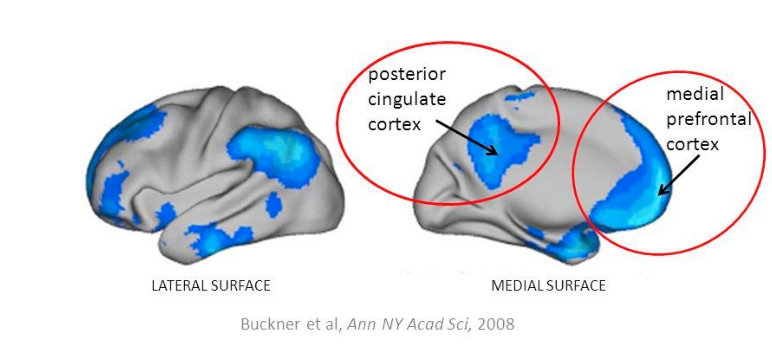
\includegraphics[height=6cm]{Pictures/DMN_anatomy.png}
    \caption{Brain regions included in DMN}
    \label{fig:my_label}
\end{figure}

The repeated observation that the ventral medial prefrontal cortex (vmPFC) and posterior cingulate cortex (PCC) paradoxically exhibit high levels of activity during resting baseline and decreases in activity during externally-oriented cognitive tasks led to the characterization of these regions as belonging to a “default mode network” (DMN) (Esposito, et al. 2006; Fransson 2006; Gusnard, et al. 2001a; McKiernan, et al. 2003; Raichle, et al. 2001). Originally proposed as a system for evaluating “information broadly arising in the external and internal milieu” (Raichle, et al. 2001), the network has since been posited to underlie a variety of functions. The DMN has been linked to episodic memory (Greicius and Menon 2004) and memory consolidation (Miall and Robertson 2006) in some studies, and social (Iacoboni, et al. 2004; Uddin, et al. 2005) or self-related processes (Buckner and Carroll 2007; Gusnard, et al. 2001a; Wicker, et al. 2003) in others. Still others associate default mode function with more general processes such as stimulus-independent (Mason, et al. 2007) or task-unrelated thought (McKiernan, et al. 2006). Though it is possible that one comprehensive theory will arise explaining the network’s ability to support such a diverse array of functions, the greater likelihood is that the default mode network consists of functionally differentiable subdivisions or subnetworks.

\paragraph{Posterior cingulate cortex (PCC) $\And$ precuneus: } The ventral (lower) part of PCC activates in all tasks related to the self, related to others, remembering the past, thinking about future, and processing concepts plus spatial navigation. The dorsal (upper) part of PCC involves involuntary awareness and arousal. [FIGURE 1.4]
% \begin{figure}
%     \centering
%     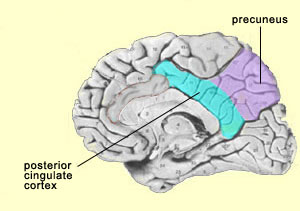
\includegraphics[height=7cm]{Pictures/pcc.jpg}
%     \caption{Posterior cingulate cortex (PCC) $\And$ precuneus }
%     \label{fig:my_label}
% \end{figure}

\paragraph{Medial prefrontal cortex (mPFC):} Decisions about self processing such as personal information, autobiographical memories, future goals and events, and decision making regarding those personally very close such as family. . [FIGURE 1.4]

\paragraph{Angular gyrus:} Connects perception, attention, spatial cognition, and action and helps with parts of recall of episodic memories.The angular gyrus is a region of the brain in the parietal lobe, that lies near the superior edge of the temporal lobe, and immediately posterior to the supramarginal gyrus; it is involved in a number of processes related to language, number processing and spatial cognition, memory retrieval, attention, and theory of mind. . [FIGURE 1.3]


\section{Data set}
The data set we are using has been collected during an another study [3].So, i am describing the method of data collection here of that data.
\paragraph{Subjects :}
   Two participants S1 female (age 25) and S2 male (age 31) volunteered for this experiment after providing written informed consent.Both participants had normal or corrected to normal vision. They were both right handed and reported no mental or neurological disorder. The two subjects did not receive any monetary compensation for their participation. The experimental protocol was approved by the local ethical committee (CPP 2010-A00744-35). Both subjects had performed the task before and had been practicing meditation.To accumulate enough mind wandering data, each subject performed 10 sessions of 20 min each over the course of about 5 weeks.
\paragraph{Procedure:}
    Subjects sat in a dimly lit room with their heads on a chin rest. Instructions were displayed at the beginning of each session on the screen placed at 60 cm in front of them.The task of the subjects was to count backward each of their breath cycles (inhale/exhale) from 10 to 1. At 1, they were instructed to restart counting backward from 10.Subjects also had to indicate whenever they realized they had lost track of their breath count (i.e., that their attention had drifted) by pressing the left mouse button.Immediately following the button press, a short 1-page phenomenological questionnaire was presented on the computer screen. The questionnaire allowed the subject to characterize their mind wandering episodes. After the questionnaire was completed, subjects had to press the right mouse button to indicate they were ready to restart the breath counting task.EEG data were recorded using a 64-channel Bio-semi Active Two system.
    
\section{Data processing}
 Data is collected using EEG.It also contains alert state data along with mind wandering state data.So, we have to select only mind-wandering state data.And to see the desired result we have to follow some steps that are shown in Figure 1.5.  
 \begin{figure}
    \centering
    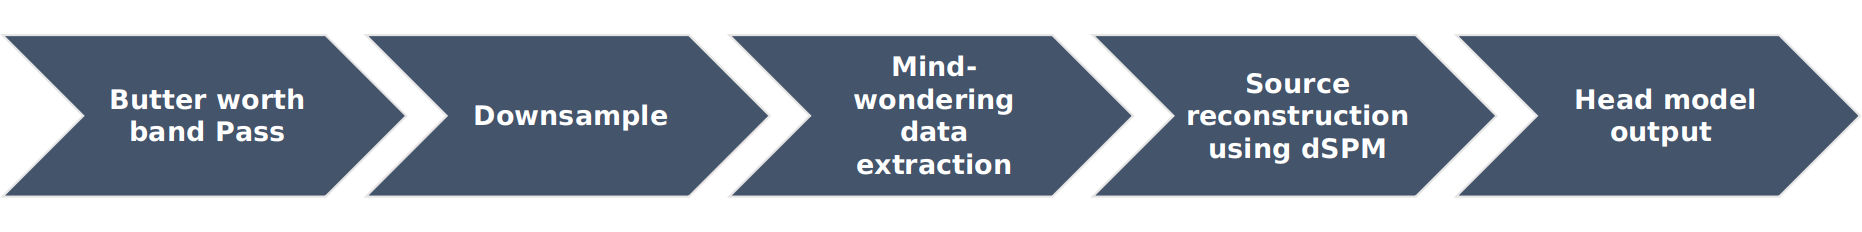
\includegraphics[width=15cm]{Pictures/Picture2.png}
    \caption{Steps of data processing}
    \label{fig:my_label1}
\end{figure}
\subsection{Prepocessing}
    \paragraph{Band Pass Butter worth filtering:} By comparing source  activation levels, we found $\theta$- and $\alpha$ band power changes in the medial prefrontal cortex, the posterior cingulate cortex, and the temporoparietal junction - a pattern that is highly consistent with the DMN. So,for our study we are focusing on the $\theta$ -band (3.5Hz-7Hz) and $\alpha$ -band (8-14 Hz).We restricted our analysis to a combination of $\theta$ and $\alpha$ frequency bands (4–16 Hz, individually adjusted for each subject). The lower $\theta$ boundary was set to 4 Hz for all the subjects, while the upper $\alpha$ boundary was set to 14Hz.
    \paragraph{Down sampling :}
    The data was then band-pass filtered with a 3rd order Butter-worth filter in the $\theta$-and in the $\alpha$- frequency band, respectively.The sampling rate of original data was 1024Hz.With this sampling rate it was not quite possible to process data further.SO,we have down-sampled data to 256 Hz.We decided down-sampling rate  by keeping information loss factor in mind. 
    \paragraph{Mind wandering data extraction:}
    The data was collected continuously.SO, it was contaminated with alertness data.During the data collection subjects had to press button when they realized that they were lost.So, we considered that it took 2 seconds of time to realize and press the button.And we also considered that subject was in mind-wandering state at least for 4 seconds.For mind-wandering data, we extracted data from -6 to -2 seconds where button press event occured at 0 second.

\subsection{Source reconstruction using dSPM}
    To project the sensor activation on the source level, we applied Dynamic Statistical Parametric Mapping,a noise-normalized minimum norm estimate, to the preprocessed data.We generated the forward model with the BrainStorm toolbox,using standardized electrode locations and a standardized three-shell spherical head model. Then, the activity of each source was estimated from the measurements of the electrical potential on the surface of the scalp at all electrodes.We then estimated a noise-normalized current dipole power at each time point and location . We made no assumptions on dipole orientation and thus averaged three dipoles for each location:

\section{Results}

\begin{figure}
    \centering
    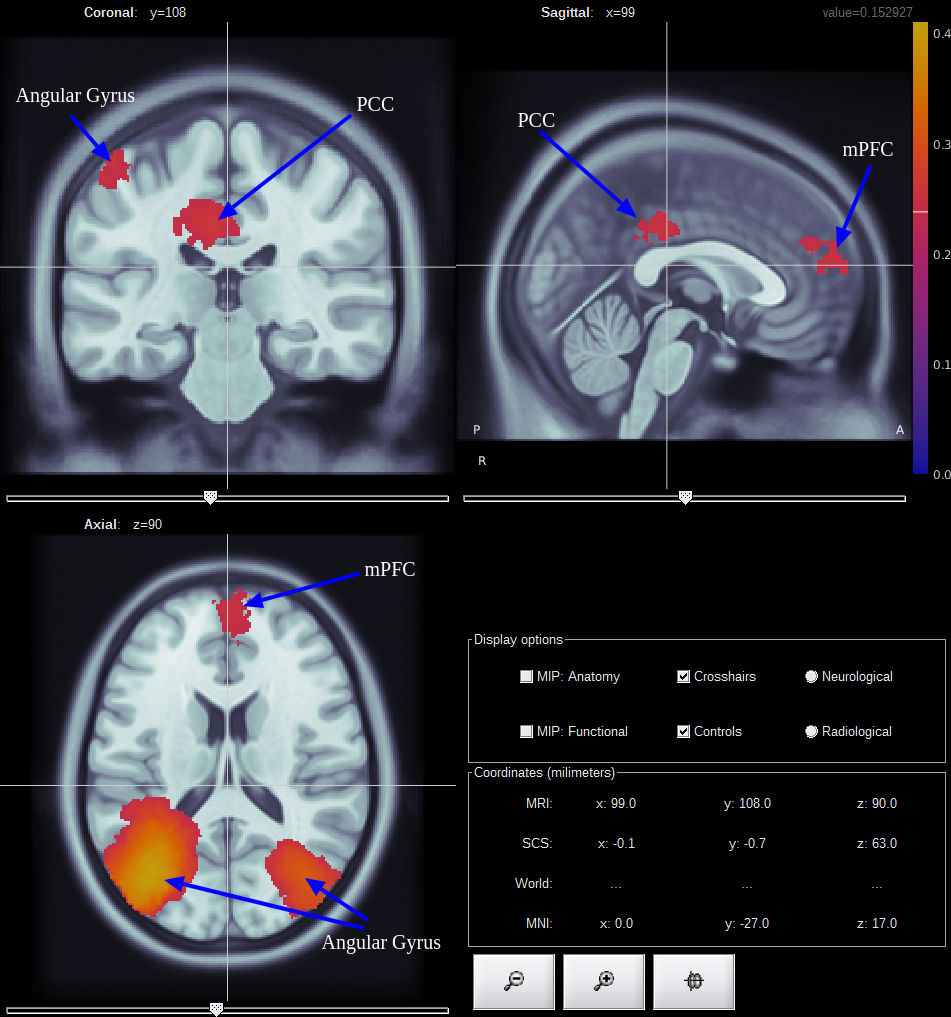
\includegraphics[width=15cm]{Pictures/result1.png}
    \caption{The Default Mode Network (DMN) identified with EEG.Orange shows positive correlation with
the autobiographical memories condition}
    \label{fig:my_label3}
\end{figure}
Figure 1.6 displays the sources that we found to show a statistically significant modulation on the group-level. We find the most prominent modulation of band power in the posterior cingulate cortex (PCC),which constitutes a hub of the DMN . In addition, we observe band power modulation in the medial prefrontal cortex (mPFC) and in the left temporoparietal junction. With the exception of the right temporoparietal junction, our method thus identifies the core areas of the DMN.

\section{Discussion}
We identified a pattern of EEG band power modulation consistent with the characterization of  DMN with PET and fMRI using the cognitive strategy of alternating autobiographical memories and focusing on breathing. For two reasons, this is particularly important. First, this EEG-based identification of DMNs enables us to study the oscillatory properties of DMNs that are not accessible by PET or fMRI. And second, our work makes it possible to study DMN changes in the patient.

Nevertheless, we note that, despite the fact that fMRI has a higher spatial resolution, the EEG-based DMN nodes are smaller than those identified by fMRI. The low spatial resolution of EEG source localization methods is one potential reason for this observation. The spatial variation between individual DMN patterns may be smaller than each individual DMN pattern on its own due to differences in head shape and cortical folding between subjects. This can contribute to a spatial underestimation of the DMN at group level. Using individualized EEG forward models derived from structural MRI scans may address this problem.
% \begin{figure}
% \centering
% 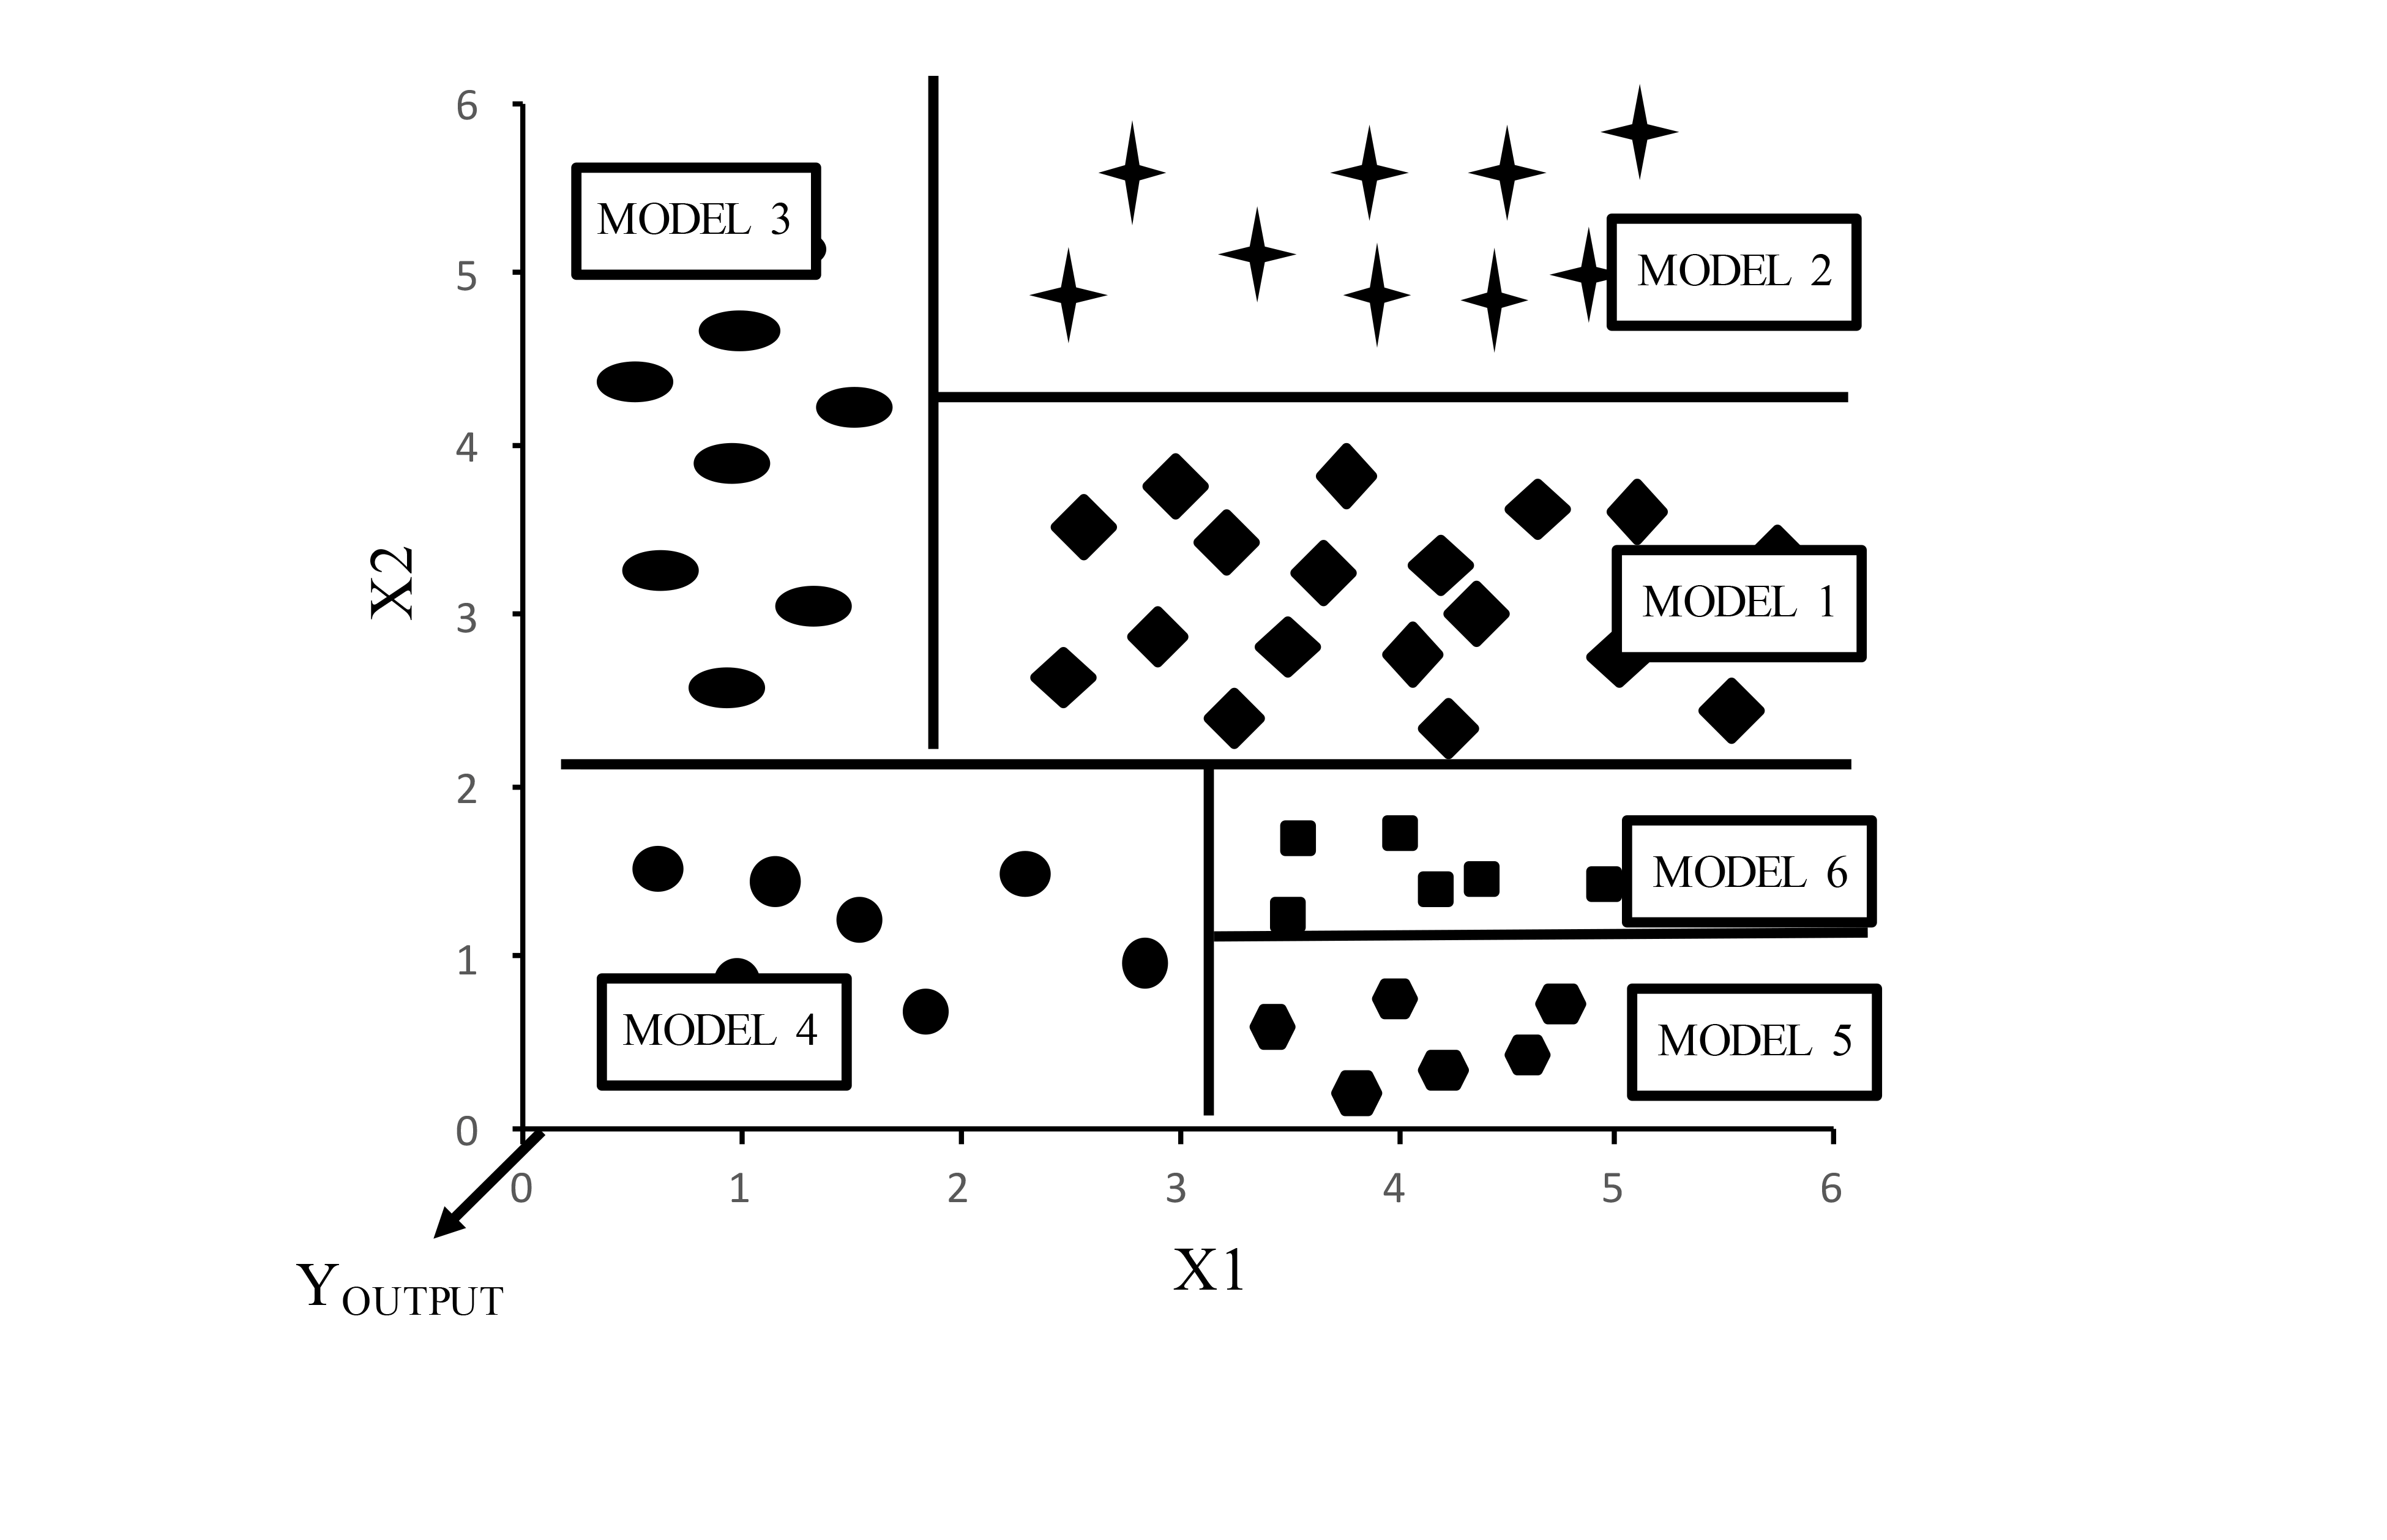
\includegraphics[height=7cm]{splits.png}
% \caption{Splitting of the input space (X1 x X2) by M5' model tree algorithm}
% \label{fig7}
% \end{figure}

% \section{Adding another section}
% You can show a lot of figures together like these Figures \ref{fig61}, \ref{fig62}, \ref{fig63} below.
% \begin{figure} [!htbp]
% \centering    
% \subfigure[Caption1]{\label{fig61}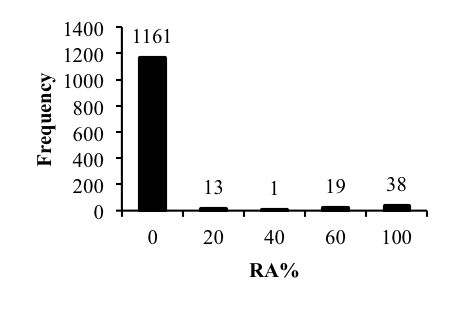
\includegraphics[width=42mm]{data1.png}}
% \subfigure[Caption2]{\label{fig62}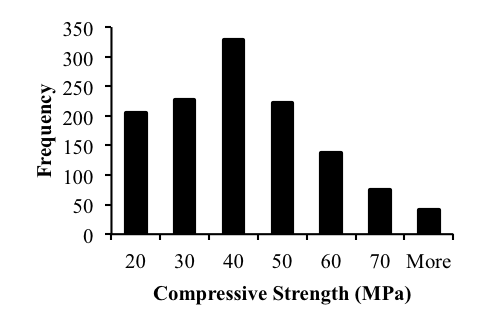
\includegraphics[width=42mm]{data2.png}}
% \subfigure[Caption3]{\label{fig63}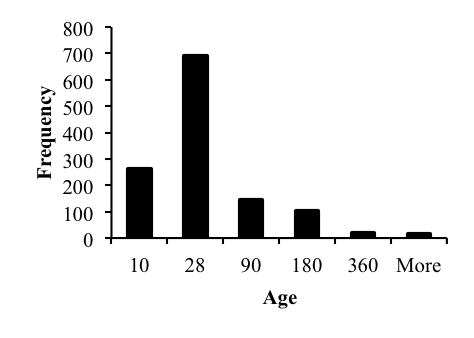
\includegraphics[width=42mm]{data3.png}}
% \caption{Figures sample}
% \end{figure}
% You can add lists into the text like this. 
% \begin{itemize}
% \settowidth{\leftmargin}{{\Large$\square$}}\advance\leftmargin\labelsep
% \itemsep3pt\relax
% \renewcommand\labelitemi{{\lower1pt\hbox{\small$\square$}}}
% \item	Some sample text item 1. 
% \item You may refer to tables \ref{tab1} 
% \item Or figures \ref{fig61}
% \end{itemize}

% Tables can be added like this
% \begin{table}[!htbp]
% \centering
% \caption{Sample table}
% \label{tab1}
% \begin{tabular}{llll}

% \hline
% Column 1 & Column 2 & Column 3       \\\hline
% 1         & Data1 & 13.41179 & 0.9492839 \\
% 2            & Data2 & 13.39824 & 0.9492952\\\hline
% \end{tabular}
% \end{table}


